\documentclass[tikz,border=1mm]{standalone}
\usetikzlibrary{matrix,chains,positioning,decorations.pathreplacing,arrows}

% Code modified from here https://tex.stackexchange.com/questions/505741/architecture-neural-network-with-weights

\begin{document}
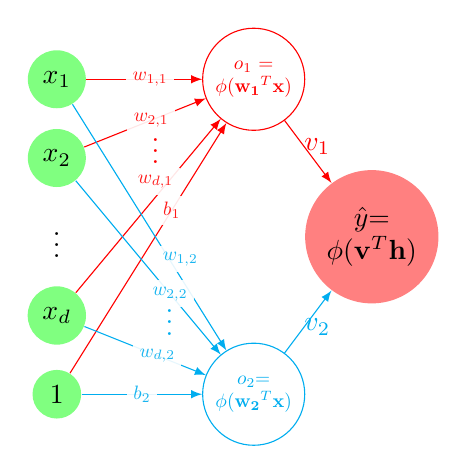
\begin{tikzpicture}[>=latex]
\path
(0,2)     node[circle,draw,red, align=center, scale=0.7] (S1) {$o_1$ =\\ $\phi(\mathbf{w_1}^T\mathbf{x})$}
% +(90:2) node[circle,draw,inner sep=2.5pt] (b) {}
%           node[above=1mm] {$b_1$}
+(-2.5,0)  node[circle,fill=green!50]  (x1) {$x_1$}
+(-2.5,-1)    node[circle,fill=green!50]  (x2) {$x_2$}
+(-2.5,-2) node  ()  {$\vdots$}
+(-2.5,-3) node[circle,fill=green!50]  (xd) {$x_d$}
+(-2.5,-4) node[circle,fill=green!50]  (b) {$1$}

(0,-2)     node[circle,draw,cyan,  align=center, scale=0.7] (S2) {$o_2$=\\ $\phi(\mathbf{w_2}^T\mathbf{x})$}

(1.5,0)  node[circle,fill=red!50, align=center]  (y) {$\hat{y}$=\\ $\phi(\mathbf{v}^T\mathbf{h})$};

\draw[->, red] (b)--(S1) node[pos=.65, fill=white, opacity=.9, scale=0.7]{$b_{1}$};
\draw[->, red] (x1)--(S1) node[pos=.55,fill=white, opacity=.9, scale=0.7]{$w_{1,1}$};
\draw[->, red] (x2)--(S1) node[pos=.55,fill=white, opacity=.9, scale=0.7]{$w_{2,1}$}; 
\draw[->, red] (xd)--(S1) node[pos=.55,fill=white, opacity=.9, scale=0.7, above=.2mm]{$w_{d,1}$} node[pos=.55,above=3mm]{$\vdots$};

\draw[->, cyan] (x1)--(S2) node[pos=.7,fill=white, opacity=.9, scale=0.7, above=.5mm]{$w_{1,2}$};
\draw[->, cyan] (x2)--(S2) node[pos=.65,,fill=white, opacity=.9, scale=0.7]{$w_{2,2}$}; 
\draw[->, cyan] (xd)--(S2) node[pos=.6,,fill=white, opacity=.9, scale=0.7]{$w_{d,2}$} node[pos=.7,above=2mm]{$\vdots$};
\draw[->, cyan] (b)--(S2) node[pos=.5,fill=white, opacity=.9, scale=0.7]{$b_{2}$};

\draw[->, red] (S1)--(y) node[pos=.7,above]{$v_{1}$};
\draw[->, cyan] (S2)--(y) node[pos=.7,below]{$v_{2}$};

% \draw[blue] (0.7,0) circle(1.5);

% \draw[decorate,decoration={brace,mirror}] (x1.west) -- node[left=10pt] {Inputs} (xd.west);
\end{tikzpicture}
\end{document}
